\printconcepts

\exercise{In your own words, describe how to plot the polar point $P(r,\theta)$.}{Answers will vary.}

\exercise{T/F: When plotting a point with polar coordinate $P(r,\theta)$, $r$ must be positive.}{F}

\exercise{T/F: Every point in the Cartesian plane can be represented by a polar coordinate.}{T}

\exercise{T/F: Every point in the Cartesian plane can be represented uniquely by a polar coordinate.}{F}

\printproblems

\exercise{Plot the points with the given polar coordinates.\\
\begin{minipage}[t]{.5\linewidth}
\begin{enumerate}
	\item $A=P(2,0)$
	\item	$B=P(1,\pi)$
\end{enumerate}
\end{minipage}%
\begin{minipage}[t]{.5\linewidth}
\begin{enumerate}\addtocounter{enumii}{2}
	\item $C=P(-2,\pi/2)$
	\item	$D=P(1,\pi/4)$
\end{enumerate}
\end{minipage}
}{\begin{minipage}[m]{\linewidth}
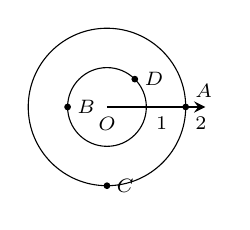
\begin{tikzpicture}[scale=.5]
	\foreach \x in {1,2}
	{\draw (0,0) circle (\x);
		\draw (\x,0) node [below right] {\scriptsize $\x$};
	}
	\draw [thick,->,>=stealth] (0,0) node [below] {\scriptsize $O$} -- (2.5,0);
	\filldraw (xyz polar cs: angle=0,radius=2) circle (2pt) node [above right] {\scriptsize $A$}
	      (xyz polar cs: angle=180,radius=1)circle (2pt) node [right] {\scriptsize $B$}
				(xyz polar cs: angle=90,radius=-2)circle (2pt) node [right] {\scriptsize $C$}
				(xyz polar cs: angle=45,radius=1)circle (2pt) node [right] {\scriptsize $D$};
	\end{tikzpicture}
\end{minipage}}

\exercise{Plot the points with the given polar coordinates.\\
\begin{minipage}[t]{.5\linewidth}
\begin{enumerate}
	\item $A=P(2,3\pi)$
	\item	$B=P(1,-\pi)$
\end{enumerate}
\end{minipage}%
\begin{minipage}[t]{.5\linewidth}
\begin{enumerate}\addtocounter{enumii}{2}
	\item $C=P(1,2)$
	\item	$D=P(1/2,5\pi/6)$
\end{enumerate}
\end{minipage}
}{\begin{minipage}[m]{\linewidth}
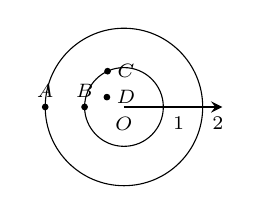
\begin{tikzpicture}[scale=.5]
	\foreach \x in {1,2}
	{\draw (0,0) circle (\x);
		\draw (\x,0) node [below right] {\scriptsize $\x$};
	}
	\draw [thick,->,>=stealth] (0,0) node [below] {\scriptsize $O$} -- (2.5,0);
	\filldraw (xyz polar cs: angle=180,radius=2) circle (2pt) node [above] {\scriptsize $A$}
	      (xyz polar cs: angle=180,radius=1)circle (2pt) node [above] {\scriptsize $B$}
				(xyz polar cs: angle=114.6,radius=1)circle (2pt) node [right] {\scriptsize $C$}
				(xyz polar cs: angle=150,radius=.5)circle (2pt) node [right] {\scriptsize $D$};
	\end{tikzpicture}
\end{minipage}}

\exercise{For each of the given points give two sets of polar coordinates that identify it, where $0\leq \theta\leq 2\pi$.

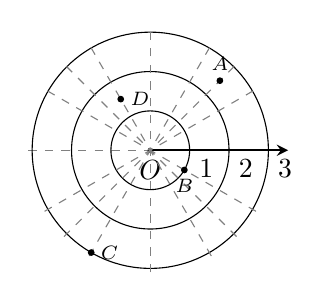
\begin{tikzpicture}[scale=.5]
	\draw [dashed,gray] (-3.1,0) -- (0,0);
	\draw[thick,->,>=stealth] (0,0) node [below] {$O$} -- (3.5,0) ;
	\filldraw (0,0) circle (1.5pt);
	\foreach \x in {1,2,3}
	{\draw (0,0) circle (\x cm);
	\draw (\x,0) node [below right] {\x};
	}
	\foreach \x in {30,45,60,90,120,135,150}
	{\draw [rotate=\x,dashed,gray] (-3.1,0) -- (3.1,0);
	}
	\filldraw (xyz polar cs: angle=45,radius=2.5) circle (2pt) node [above] {\scriptsize $A$}
	      (xyz polar cs: angle=-30,radius=1)circle (2pt) node [below] {\scriptsize $B$}
				(xyz polar cs: angle=240,radius=3)circle (2pt) node [right] {\scriptsize $C$}
				(xyz polar cs: angle=120,radius=1.5)circle (2pt) node [right] {\scriptsize $D$};
	
\end{tikzpicture}	
}{$A=P(2.5,\pi/4)$ and $P(-2.5,5\pi/4)$;\\
$B=P(-1,5\pi/6)$ and $P(1,11\pi/6)$;\\
$C=P(3,4\pi/3)$ and $P(-3,\pi/3)$;\\
$D=P(1.5,2\pi/3)$ and $P(-1.5,5\pi/3)$}

\exercise{For each of the given points give two sets of polar coordinates that identify it, where $-\pi\leq \theta\leq \pi$.

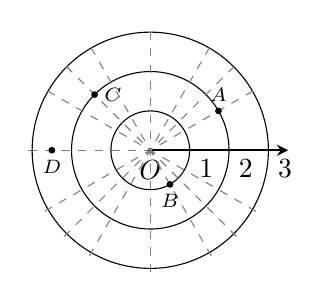
\begin{tikzpicture}[scale=.5]
	\draw [dashed,gray] (-3.1,0) -- (0,0);
	\draw[thick,->,>=stealth] (0,0) node [below] {$O$} -- (3.5,0) ;
	\filldraw (0,0) circle (1.5pt);
	\foreach \x in {1,2,3}
	{\draw (0,0) circle (\x cm);
	\draw (\x,0) node [below right] {\x};
	}
	\foreach \x in {30,45,60,90,120,135,150}
	{\draw [rotate=\x,dashed,gray] (-3.1,0) -- (3.1,0);
	}
	\filldraw (xyz polar cs: angle=30,radius=2) circle (2pt) node [above] {\scriptsize $A$}
	      (xyz polar cs: angle=-60,radius=1)circle (2pt) node [below] {\scriptsize $B$}
				(xyz polar cs: angle=135,radius=2)circle (2pt) node [right] {\scriptsize $C$}
				(xyz polar cs: angle=180,radius=2.5)circle (2pt) node [below] {\scriptsize $D$};
	
\end{tikzpicture}	
}{$A=P(2,\pi/6)$ and $P(-2,-5\pi/6)$;\\
$B=P(1,-\pi/3)$ and $P(-1,2\pi/3)$;\\
$C=P(2,3\pi/4)$ and $P(-2,-\pi/4)$;\\
$D=P(2.5,\pi)$ and $P(2.5,-\pi)$}

\exercise{Convert each of the following polar coordinates to rectangular, and each of the following rectangular coordinates to polar.\\
\begin{minipage}[t]{.5\linewidth}
\begin{enumerate}
	\item $A=P(2,\pi/4)$
	\item $B=P(2,-\pi/4)$
\end{enumerate}
\end{minipage}%
\begin{minipage}[t]{.5\linewidth}
\begin{enumerate}\addtocounter{enumii}{2}
	\item $C=(2,-1)$
	\item $D=(-2,1)$
\end{enumerate}
\end{minipage}
}{$A=(\sqrt{2},\sqrt{2})$;\\
$B=(\sqrt{2},-\sqrt{2})$;\\
$C=P(\sqrt{5},-0.46)$;\\
$D=P(\sqrt{5},2.68)$}

\exercise{Convert each of the following polar coordinates to rectangular, and each of the following rectangular coordinates to polar.\\
\begin{minipage}[t]{.5\linewidth}
\begin{enumerate}
	\item $A=P(3,\pi)$
	\item $B=P(1,2\pi/3)$
\end{enumerate}
\end{minipage}%
\begin{minipage}[t]{.5\linewidth}
\begin{enumerate}\addtocounter{enumii}{2}
	\item $C=(0,4)$
	\item $D=(1,-\sqrt{3})$
\end{enumerate}
\end{minipage}
}{$A=(-3,0)$;\\
$B=(-1/2,\sqrt{3}/2)$;\\
$C=P(4,\pi/2)$;\\
$D=P(2,-\pi/3)$}

\exerciseset{In Exercises}{, graph the polar function on the given interval.
}{

\exercise{$r=2$,\quad $0\leq \theta\leq \pi/2$
}{\noindent\begin{minipage}[m]{\linewidth}
\myincludegraphics[scale=.75]{figures/fig09_04_ex_11}
\end{minipage}
}

\exercise{$\theta=\pi/6$,\quad $-1\leq r\leq 2$
}{\noindent\begin{minipage}[m]{\linewidth}
\myincludegraphics[scale=.75]{figures/fig09_04_ex_12}
\end{minipage}
}

\exercise{$r=1-\cos \theta$,\quad $[0,2\pi]$
}{\noindent\begin{minipage}[m]{\linewidth}
\myincludegraphics[scale=.75]{figures/fig09_04_ex_13}
\end{minipage}
}

\exercise{$r=2+\sin \theta$,\quad $[0,2\pi]$
}{\noindent\begin{minipage}[m]{\linewidth}
\myincludegraphics[scale=.75]{figures/fig09_04_ex_14}
\end{minipage}
}

\exercise{$r=2-\sin \theta$,\quad $[0,2\pi]$
}{\noindent\begin{minipage}[m]{\linewidth}
\myincludegraphics[scale=.75]{figures/fig09_04_ex_15}
\end{minipage}
}

\exercise{$r=1-2\sin \theta$,\quad $[0,2\pi]$
}{\noindent\begin{minipage}[m]{\linewidth}
\myincludegraphics[scale=.75]{figures/fig09_04_ex_16}
\end{minipage}
}

\exercise{$r=1+2\sin \theta$,\quad $[0,2\pi]$
}{\noindent\begin{minipage}[m]{\linewidth}
\myincludegraphics[scale=.75]{figures/fig09_04_ex_17}
\end{minipage}
}

\exercise{$r=\cos(2\theta)$,\quad $[0,2\pi]$
}{\noindent\begin{minipage}[m]{\linewidth}
\myincludegraphics[scale=.75]{figures/fig09_04_ex_18}
\end{minipage}
}

\exercise{$r=\sin(3\theta)$,\quad $[0,\pi]$
}{\noindent\begin{minipage}[m]{\linewidth}
\myincludegraphics[scale=.75]{figures/fig09_04_ex_19}
\end{minipage}
}

\exercise{$r=\cos(\theta/3)$,\quad $[0,3\pi]$
}{\noindent\begin{minipage}[m]{\linewidth}
\myincludegraphics[scale=.75]{figures/fig09_04_ex_20}
\end{minipage}
}

\exercise{$r=\cos(2\theta/3)$,\quad $[0,6\pi]$
}{\noindent\begin{minipage}[m]{\linewidth}
\myincludegraphics[scale=.75]{figures/fig09_04_ex_21}
\end{minipage}
}

\exercise{$r=\theta/2$,\quad $[0,4\pi]$
}{\noindent\begin{minipage}[m]{\linewidth}
\myincludegraphics[scale=.75]{figures/fig09_04_ex_22}
\end{minipage}
}

\exercise{$r=3\sin(\theta)$,\quad $[0,\pi]$
}{\noindent\begin{minipage}[m]{\linewidth}
\myincludegraphics[scale=.75]{figures/fig09_04_ex_23}
\end{minipage}
}

\exercise{$r=\cos\theta\sin\theta$,\quad $[0,2\pi]$
}{\noindent\begin{minipage}[m]{\linewidth}
\myincludegraphics[scale=.75]{figures/fig09_04_ex_24}
\end{minipage}
}

\exercise{$r=\theta^2-(\pi/2)^2$,\quad $[-\pi,\pi]$
}{\noindent\begin{minipage}[m]{\linewidth}
\myincludegraphics[scale=.75]{figures/fig09_04_ex_25}
\end{minipage}
}

\exercise{$\ds r=\frac{3}{5\sin\theta-\cos\theta}$,\quad $[0,2\pi]$
}{\noindent\begin{minipage}[m]{\linewidth}
\myincludegraphics[scale=.75]{figures/fig09_04_ex_26}
\end{minipage}
}

\exercise{$\ds r=\frac{-2}{3\cos\theta-2\sin\theta}$,\quad $[0,2\pi]$
}{\noindent\begin{minipage}[m]{\linewidth}
\myincludegraphics[scale=.75]{figures/fig09_04_ex_27}
\end{minipage}
}

\exercise{$\ds r=3\sec \theta$,\quad $(-\pi/2,\pi/2)$
}{\noindent\begin{minipage}[m]{\linewidth}
\myincludegraphics[scale=.75]{figures/fig09_04_ex_28}
\end{minipage}
}

\exercise{$\ds r=3\csc \theta$,\quad $(0,\pi)$
}{\noindent\begin{minipage}[m]{\linewidth}
\myincludegraphics[scale=.75]{figures/fig09_04_ex_29}
\end{minipage}
}
}

\exerciseset{In Exercises}{, convert the  polar equation to a rectangular equation.}{

\exercise{$r=2\cos\theta$}{$(x-1)^2+y^2=1$}

\exercise{$r=-4\sin\theta$}{$x^2+(y+2)^2=4$}

\exercise{$r=3\sin(\theta)$}{$x^2 +(y-\frac{3}{2})^2 = \frac{9}{4}$}

\exercise{$r=-\dfrac{3}{2}\cos(\theta)$}{$(x+\frac{3}{4})^2+y^2 = \frac{9}{16}$}

\exercise{$r=\cos\theta+\sin\theta$}{$(x-1/2)^2+(y-1/2)^2=1/2$}

\exercise{$r=\dfrac{7}{5\sin\theta-2\cos\theta}$}{$y=2/5x+7/5$}

\exercise{$r=\dfrac{3}{\cos\theta}$}{$x=3$}

\exercise{$r=\dfrac{4}{\sin\theta}$}{$y=4$}

\exercise{$r=\tan\theta$}{$x^4+x^2y^2x^2-y^2=0$}

\exercise{$r=2$}{$x^2+y^2=4$}

\exercise{$\theta=\dfrac\pi6$}{$y=x/\sqrt{3}$}

}


%\ifthenelse{\boolean{printquestions}}{\columnbreak}{}

\input{exercises/09_04_exset_03}

\exerciseset{In Exercises}{, find the points of intersection of the polar graphs.
}{

\exercise{$r=\sin(2\theta)$ and $r=\cos\theta$ on $[0,\pi]$}{$P(\sqrt{3}/2,\pi/6)$, $P(0,\pi/2)$, $P(-\sqrt{3}/2,5\pi/6)$
}

\exercise{$r=\cos(2\theta)$ and $r=\cos\theta$ on $[0,\pi]$}{$P(1,0)$, $P(0,\pi/2)=P(0,\pi/4)$, $P(-1/2,\pi/3)$
}

\exercise{$r=2\cos\theta$ and $r=2\sin\theta$ on $[0,\pi]$}{$P(0,0)=P(0,\pi/2)$, $P(\sqrt{2},\pi/4)$
}

\exercise{$r=\sin\theta$ and $r=\sqrt{3}+3\sin\theta$ on $[0,2\pi]$}{$P(\sqrt{3}/2,\pi/3)=P(-\sqrt{3}/2,4\pi/3)$, $P(\sqrt{3}/2,2\pi/3)=P(-\sqrt{3}/2,5\pi/3)$, $P(0,\pi/2)$
}

\exercise{$r=\sin(3\theta)$ and $r=\cos(3\theta)$ on $[0,\pi]$}{$P(\sqrt{2}/2,\pi/12)$, $P(-\sqrt{2}/2,5\pi/12)$, $P(\sqrt{2}/2,3\pi/4)$
}

\exercise{$r=3\cos\theta$ and $r=1+\cos\theta$ on $[-\pi,\pi]$}{$P(3/2,\pi/3)$, $P(3/2,-\pi/3)$
}

\exercise{$r=1$ and $r=2\sin(2\theta)$ on $[0,2\pi]$}{For all points, $r=1$; $\theta = \pi/12,\ 5\pi/12,\ 7\pi/12,\ 11\pi/12,\ 13\pi/12,\ 17\pi/12,\ 19\pi/12,\ 23\pi/12$. 
}

\exercise{$r=1-\cos\theta$ and $r=1+\sin\theta$ on $[0,2\pi]$}{$P(0,0)=P(0,3\pi/2)$,  $P(1+\sqrt{2}/2,3\pi/4)$, $P(1-\sqrt{2}/2,7\pi/4)$
}
}

\exercise{Pick a integer value for $n$, where $n\neq 2,3$, and use technology to plot $\ds r=\sin\left(\frac mn\theta\right)$ for three different integer values of $m$. Sketch these and determine a minimal interval on which the entire graph is shown.}{Answers will vary. If $m$ and $n$ do not have any common factors, then an interval of $2n\pi$ is needed to sketch the entire graph.
}

\exercise{Create your own polar function, $r=f(\theta)$ and sketch it. Describe why the graph looks as it does.}{Answers will vary.
}
